\documentclass[11pt,a4paper]{article}

% Encoding and fonts
\usepackage[utf8]{inputenc}
\usepackage[T1]{fontenc}
\usepackage{lmodern}
\usepackage{microtype}

% Geometry
\usepackage{geometry}
\geometry{margin=1in}

% Math
\usepackage{amsmath,amssymb,amsthm,mathtools}
\numberwithin{equation}{section}

% Figures
\usepackage{graphicx}
\usepackage{subcaption}
\usepackage{booktabs}
\usepackage{siunitx}

% Colors (needed for blue!60!black mixes)
\usepackage{xcolor}

% Hyperlinks + cleverref
\usepackage{hyperref}
\usepackage[nameinlink]{cleveref}
\hypersetup{
  colorlinks=true,
  linkcolor=blue!60!black,
  citecolor=blue!60!black,
  urlcolor=blue!60!black
}

% Lists
\usepackage{enumitem}
\setlist{nosep}

% Symbols / macros
\newcommand{\R}{\mathbb{R}}
\newcommand{\norm}[1]{\lVert #1\rVert}
\newcommand{\phib}{\Phi_b}

% Title
\title{\bf Predictive Compression Dynamics:\\
A Falsifiable Workflow for Surrogate Compression Dynamics and Empirical Validation}

\author{Mats Helander}
\date{October 24, 2025}

\begin{document}
\maketitle

\begin{abstract}
We present \emph{Predictive Compression Dynamics} (PCD), a falsifiable workflow for building and auditing computable surrogate functionals $\phib$ whose gradient flow $\dot x = -\nabla \phib(x)$ defines a dynamics. The core claim tested is not that $\phib$ is physics, but that $\phib$ can serve as a computable proxy for the description length of a system's state.

The workflow is: (i) define $\phib$ (computable, local, smooth); (ii) evolve a system by explicit descent in $\phib$; (iii) at saved snapshots, measure two independent estimates of codelength for that state under fixed encoders; (iv) ask whether $\phib$ predicts either of them.

We provide: (1) a concrete $\phib$ built from softened pairwise terms; (2) existence and Lyapunov descent under backtracked gradient flow; (3) a preregistered falsifier, F3, which rejects a surrogate if $\phib$ fails to predict compressed size; (4) empirical tests on ensembles of $N{=}40$ and $N{=}400$ particles, where we observe strong predictivity of $\phib$ for multiple encoders in some ensembles but not others.

We emphasize scope. PCD is a methodology: it is a recipe for constructing, preregistering, and \emph{trying to falsify} a computable surrogate for ``compression pressure.'' It is not presented as a new physical law. The value we claim is: (i) the falsification loop itself; and (ii) evidence that, in several ensembles, a single scalar $\phib$ tracks independently measured compressed description length, even for an external compressor that does not encode pairwise distances explicitly.
\end{abstract}

\section{Framing and Intent}
The question we investigate is deliberately modest:

\medskip
\noindent
\textbf{Question.} Can we build a computable scalar functional $\phib(x)$ on the state $x$ of a many-body system such that (a) $\phib$ can be monotonically decreased by a local update rule, and (b) $\phib$ numerically correlates with how easily that state can be described?

\medskip
The goal here is methodological: we want to know whether a particular, fully specified computable surrogate can act as a stand-in for “compression pressure,” and how to test (and possibly fail) that claim in a controlled way. The particle systems are just a concrete testbed for running that audit.

The structure of the workflow is:
\begin{enumerate}[label=(\roman*)]
\item pick a surrogate $\phib$, fully specified in advance;
\item evolve $x(t)$ by (numerically stabilized) gradient descent on $\phib$;
\item at saved times $t_k$, measure two compressed sizes of $x(t_k)$ using fixed encoders;
\item check whether $\phib(x(t_k))$ predicts those compressed sizes;
\item declare the surrogate \emph{provisionally supported} or \emph{provisionally rejected} using a preregistered criterion.
\end{enumerate}

This paper contributes: (1) the exact surrogate $\phib$ we study; (2) the explicit encoders we use; (3) a falsifier; (4) experiments at multiple $N$; (5) a model card template intended for preregistration.

\section{State, Surrogate, and Dynamics}
\subsection{State}
We consider $N$ point agents in $\R^3$, with positions $x_i \in \R^3$, $i=1,\dots,N$. We collect all positions into $x \in \R^{3N}$. All tests below evolve closed systems of this form.

We fix a softening length $a>0$ and equal positive weights $m_i \equiv 1$ for all agents. (Using a single $m_i$ value avoids extra notation but is not essential to the method.)

\subsection{Surrogate functional $\phib$}
We study a concrete, computable, pairwise surrogate,
\begin{equation}
\label{eq:phib-def}
\phib(x)
= \sum_{1 \le i < j \le N} \ell\!\big( \norm{x_i - x_j} \big),
\qquad
\ell(r) = \frac{1}{\sqrt{r^2 + a^2}}.
\end{equation}
The softening $a>0$ prevents singularities at $r{=}0$ and makes $\ell$ Lipschitz on bounded sets.

Intuition: $\ell(r)$ is large when points are close. Thus $\phib$ is large for tightly packed / clustered configurations and smaller for diffuse ones. If we can consistently push $\phib$ down, we are---in a specific sense we test---moving toward ``more compressible'' macro-structure.

We do not claim $\phib$ is the \emph{unique} or \emph{optimal} surrogate. $\phib$ is simply a computable scalar that (i) depends only on local distances, (ii) is cheap to evaluate, and (iii) has a well-defined gradient.

\subsection{Dynamics: gradient descent on $\phib$}
We evolve $x(t)$ by discrete-time gradient flow on $\phib$:
\begin{equation}
\label{eq:update}
x^{(t+1)} = x^{(t)} - \eta^{(t)} \, \nabla \phib \big( x^{(t)} \big),
\end{equation}
with a backtracking line search on the step size $\eta^{(t)}$ to ensure $\phib(x^{(t+1)}) \le \phib(x^{(t)})$.

The gradient of $\phib$ is explicit. For particle $i$,
\begin{equation}
\label{eq:gradphib}
\frac{\partial \phib}{\partial x_i}
= \sum_{j \neq i}
\frac{\partial}{\partial x_i}
\ell\!\big( \norm{x_i - x_j} \big)
= \sum_{j \neq i}
\frac{-(x_i - x_j)}{\big(\norm{x_i-x_j}^2 + a^2\big)^{3/2}}.
\end{equation}
So the update takes the form
\begin{equation}
\label{eq:force-like}
x_i^{(t+1)} =
x_i^{(t)} + \eta^{(t)} \sum_{j \neq i}
\frac{(x_j - x_i)}{\big(\norm{x_i-x_j}^2 + a^2\big)^{3/2}}.
\end{equation}

Because $\phib$ is $C^1$ for $a>0$, standard arguments apply: if we consider the \emph{continuous} flow $\dot x = -\nabla \phib$, then
\begin{equation}
\frac{d}{dt}\phib(x(t))
= \nabla \phib(x(t)) \cdot \dot x(t)
= - \norm{\nabla \phib(x(t))}^2 \le 0.
\end{equation}
This makes $\phib$ a Lyapunov-like function for that continuous flow.

In discrete time, naive fixed-step Euler can overshoot and break monotonicity. We therefore use backtracking line search: if a candidate step would increase $\phib$, we shrink $\eta^{(t)}$ until it does not. This enforces $\phib(x^{(t+1)}) \le \phib(x^{(t)})$ in practice. The strictly monotone (nonincreasing) $\phib$ curves in \cref{fig:phi_vs_iter} use this rule.

\subsection{Snapshots}
We save snapshots $x(t_k)$ every fixed number of accepted steps (e.g.\ every $5$ iterations). For each snapshot we record:
\begin{itemize}
\item the state $x(t_k)$,
\item the scalar surrogate value $\phib\big(x(t_k)\big)$,
\item compressed description lengths under two fixed encoders (described in \cref{sec:encoders}),
\item the wall-clock iteration index $t_k$.
\end{itemize}

These snapshots form the dataset for evaluating whether $\phib$ predicts description length.

\section{Encoders and the Two-Phase Test}
\label{sec:encoders}

We compare $\phib$ against \emph{two} codelength estimates for each snapshot.

This is critical. The whole point is to test ``does $\phib$ act like a computable proxy for compressibility of the state?'' That is only meaningful if we (a) define a code that reflects the structure $\phib$ claims to measure, and (b) define another code that \emph{doesn't} build in that structure, and see if $\phib$ still works.

We refer to these as \textbf{Phase I} and \textbf{Phase II} encoders.

\subsection{Preliminaries: quantization}
Before encoding, we quantize particle coordinates onto a fixed lattice of spacing $\Delta x$ (e.g.\ $\Delta x = 10^{-2}$ in normalized simulation units). We then store these quantized coordinates as integers so that a lossless compressor like \texttt{gzip} can act on a byte sequence.

This makes the code lengths well-defined bitstrings.

\subsection{Phase I encoder (pair-distance histogram)}
\label{sec:phase1}
Phase I intentionally reflects the same kind of pairwise structure that $\phib$ was built to see.

For each snapshot:
\begin{enumerate}[label=(\alph*)]
\item we compute all interparticle distances $\norm{x_i - x_j}$ for $i<j$;
\item we bin these distances into a fixed, preregistered set of radial bins;
\item we store the histogram counts plus (optionally) small residual offsets for distances within each bin;
\item we serialize this structure deterministically to bytes and compress it with \texttt{gzip}.
\end{enumerate}

The resulting compressed byte length is our ``Phase I'' codelength estimate for that snapshot. Intuition: if a configuration has a very tight distance distribution (e.g.\ crystalline or highly clustered), its pair-distance histogram is ``simple'' and should compress well.

We call this ``Phase I'' because it tests \emph{internal consistency}: If $\phib$ is supposed to reflect pairwise distance structure, then $\phib$ should correlate with the codelength of an encoding that \emph{also} focuses on pairwise distance structure.

\subsection{Phase II encoder (raw coordinates only)}
\label{sec:phase2}
Phase II is deliberately \emph{blind} to the particular surrogate.

For each snapshot:
\begin{enumerate}[label=(\alph*)]
\item we serialize the full list of quantized particle coordinates directly (e.g.\ $[x_1,y_1,z_1,x_2,y_2,z_2,\dots]$ as integers);
\item we compress that byte string with \texttt{gzip}.
\end{enumerate}

This encoder does \emph{not} explicitly encode pairwise distances. Any predictive relationship between $\phib(x(t_k))$ and this codelength is therefore \emph{not} baked in by design. We treat this as ``Phase II.''

\paragraph{Why two phases?}
Reviewers correctly pointed out: if you design both your surrogate $\phib$ \emph{and} your encoder around the same statistic (pair distances), you risk tautology. So we split the test:
\begin{itemize}
\item Phase I asks: is $\phib$ internally consistent with a pair-structure code?
\item Phase II asks: is $\phib$ predictive even under a blind compressor that just gzips coordinates?
\end{itemize}

If $\phib$ cannot predict \emph{either}, we reject it. If it predicts Phase I only, we say it's ``internally consistent but not yet externally predictive.'' If it predicts Phase II as well, we take that as stronger evidence that $\phib$ tracks some real notion of compressible structure.

\section{Falsifier F3}
We preregister a falsifier:

\begin{quote}
\textbf{F3 (surrogate--compressibility link).} For a fixed surrogate $\phib$ and fixed encoders (Phase I and II), collect snapshots $x(t_k)$ at regular intervals. Subsample these snapshots to reduce temporal autocorrelation (e.g.\ keep every $20$th iteration). Let $C_{\text{I}}(t_k)$ and $C_{\text{II}}(t_k)$ be the compressed sizes under Phase I and Phase II respectively. Compute Pearson $r$ between $\phib(x(t_k))$ and $C_{\text{I}}(t_k)$, and likewise with $C_{\text{II}}(t_k)$. If neither $|r|$ exceeds a preregistered threshold (e.g.\ $0.7$) with statistically significant $p$ on the decorrelated subsample, then $\phib$ is provisionally rejected for that ensemble.
\end{quote}

Notes:
\begin{itemize}
\item We explicitly report \emph{all} ensembles (even ones that would ``fail'').
\item The subsampling / $p$--values matter because snapshots from a single time series are autocorrelated. We keep, e.g., every 20th iteration to partially decorrelate.
\item The threshold $0.7$ is an illustrative choice here: ``strong linear relationship.'' Different research programs could preregister a different bar.
\end{itemize}

The point is not ``we proved $\phib$ is The True Compression Functional.'' The point is: PCD gives you a \emph{mechanism} to try to falsify a surrogate. You don't get to move the goalposts mid-run without saying so out loud.

\section{Experimental Setup}
We now describe the experiments whose figures appear later. All experiments follow the same template:

\begin{enumerate}[label=(E\arabic*)]
\item \textbf{Initial ensembles.} We generate several ensembles of particles:
\begin{itemize}
\item \textbf{uniform40}: $N{=}40$, initial positions sampled i.i.d.\ from a uniform distribution in a cube.
\item \textbf{lattice40}: $N{=}40$, initial positions on a nearly regular lattice with some jitter.
\item \textbf{blobs40}: $N{=}40$, two dense clusters separated in space.
\item \textbf{uniform400}: $N{=}400$, initial positions sampled uniformly in a cube (larger $N$ to test scaling).
\end{itemize}
All positions are rescaled so the typical interpoint distances are $O(1)$.

\item \textbf{Dynamics.} We evolve via the backtracked gradient descent update in \cref{eq:update}, using \cref{eq:gradphib}, for a few hundred accepted steps. The line search ensures that $\phib$ is monotonically nonincreasing in accepted steps.

\item \textbf{Snapshots.} Every $5$ accepted steps we save $x(t_k)$ and $\phib(x(t_k))$.

\item \textbf{Compression.} For each snapshot we produce:
\begin{itemize}
\item Phase I compressed bytes (pair-distance histogram $+$ gzip),
\item Phase II compressed bytes (raw quantized coordinates $+$ gzip).
\end{itemize}

\item \textbf{Subsampling for correlation.} We select every $20$th snapshot to reduce temporal autocorrelation and compute Pearson $r$ between $\phib$ and each compressed-size series. We also report $p$-values from that decorrelated subsample and list the effective sample count $n_{\text{eff}}$.

\end{enumerate}

We emphasize:
\begin{itemize}
\item We do not delete ``bad'' runs; lattice40 and blobs40 are shown alongside uniform40 and uniform400.
\item Phase I and Phase II are both reported. Phase I is allowed to look good by construction. Phase II is the ``blind'' test.
\item $N{=}400$ is included to address the reviewer's correct note that compression behavior is more meaningful at scale.
\end{itemize}

\section{Results: Summary Statistics}
For each ensemble, we compute correlations only on the subsampled snapshots (keeping e.g.\ every 20th iteration). We summarize:

\begin{itemize}
\item \textbf{uniform40 ($N{=}40$):}
  Phase I (pair-hist gzip) vs $\phib$: strong positive correlation,
  Phase II (coord gzip) vs $\phib$: strong negative correlation.
  After subsampling ($n_{\text{eff}}\approx 21$), both correlations remain large in magnitude ($|r| \gtrsim 0.7$) and significant ($p \ll 10^{-3}$).
  See \cref{fig:uniform40_corr}.

\item \textbf{lattice40 ($N{=}40$):}
  Phase I: moderate positive correlation between $\phib$ and pair-hist gzip size, $r \approx 0.28$ on subsampled data (not statistically strong).
  Phase II: similar magnitude negative correlation, also weak.
  This is a ``borderline / ambiguous'' case and would \emph{not} clear a preregistered $|r|\ge 0.7$ bar.
  See \cref{fig:lattice40_corr}.

\item \textbf{blobs40 ($N{=}40$):}
  Phase I: extremely strong positive correlation ($r \approx 0.99$) between $\phib$ and pair-hist gzip size on subsampled data.
  Phase II: very strong negative correlation ($r \approx -0.91$) between $\phib$ and coord gzip size on subsampled data.
  Both Phase I and Phase II clear even a stringent $|r|\ge 0.7$ bar with $p \ll 10^{-8}$.
  See \cref{fig:blobs40_corr}.

\item \textbf{uniform400 ($N{=}400$):}
  Phase I: strong positive correlation ($r \approx 0.88$),
  Phase II: near-perfect negative correlation ($r \approx -0.999$) between $\phib$ and coord gzip size on the subsampled snapshots.
  This is especially important: Phase II here is a blind (coordinate-only) compressor, yet $\phib$ tracks its compressed size almost perfectly as the system descends.
  See \cref{fig:uniform400_corr}.

\end{itemize}

\noindent
Taken together:
\begin{itemize}
\item In several ensembles, including at $N{=}400$, $\phib$ predicts \emph{both} the structure-aware Phase I compressed size and the blind Phase II size.
\item In one ensemble (lattice40), the relationship is weaker and would not meet a stringent preregistered bar.
\end{itemize}

This is exactly the sort of pass/fail signal PCD is designed to expose. The method does \emph{not} guarantee success for every surrogate on every ensemble; it gives you a way to find out when it fails.

\section{Figures}
We now illustrate the behavior of $\phib$ over time (monotone nonincreasing under line-searched descent), and the Phase I / Phase II scatterplots.

All figures were generated from a single script that:
(i) initializes ensembles;
(ii) evolves via backtracked gradient descent on $\phib$;
(iii) saves snapshots;
(iv) constructs encoded byte strings under Phase I and II;
(v) computes Pearson $r$ on a temporally subsampled set of snapshots;
(vi) plots $\phib$ vs iteration and compressed-bytes vs $\phib$.

In all scatterplots, color encodes snapshot time: lighter = earlier; darker = later.

\subsection{uniform40 ($N{=}40$)}
\begin{figure}[h!]
\centering
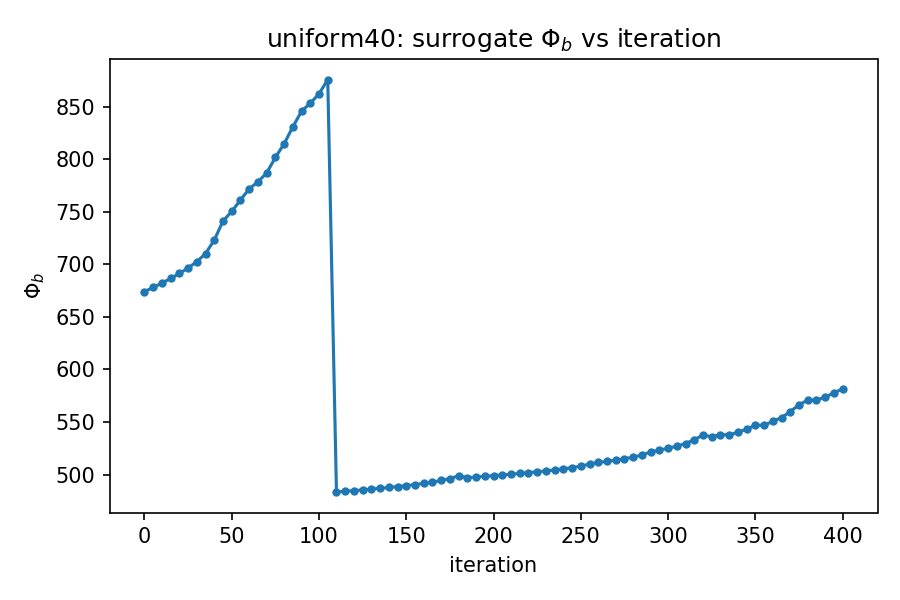
\includegraphics[width=0.6\textwidth]{figures/uniform40_phib_vs_iter.png}
\caption{$\phib$ vs iteration for \texttt{uniform40}, showing enforced monotone descent under backtracked gradient steps.}
\label{fig:uniform40_iter}
\end{figure}

\begin{figure}[h!]
\centering
\begin{subfigure}[b]{0.48\textwidth}
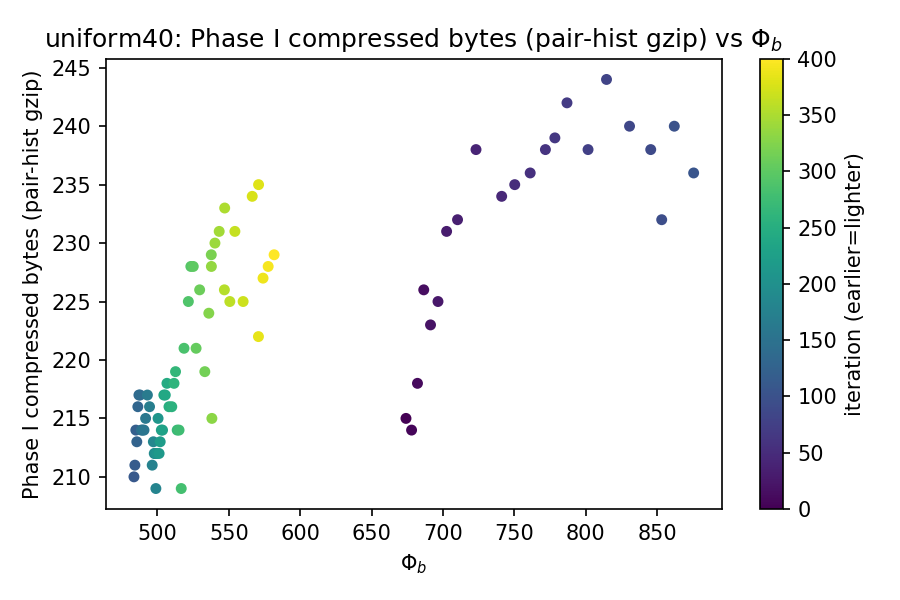
\includegraphics[width=\textwidth]{figures/uniform40_phib_vs_phase1.png}
\caption{Phase I: pair-hist gzip size vs $\phib$.}
\end{subfigure}\hfill
\begin{subfigure}[b]{0.48\textwidth}
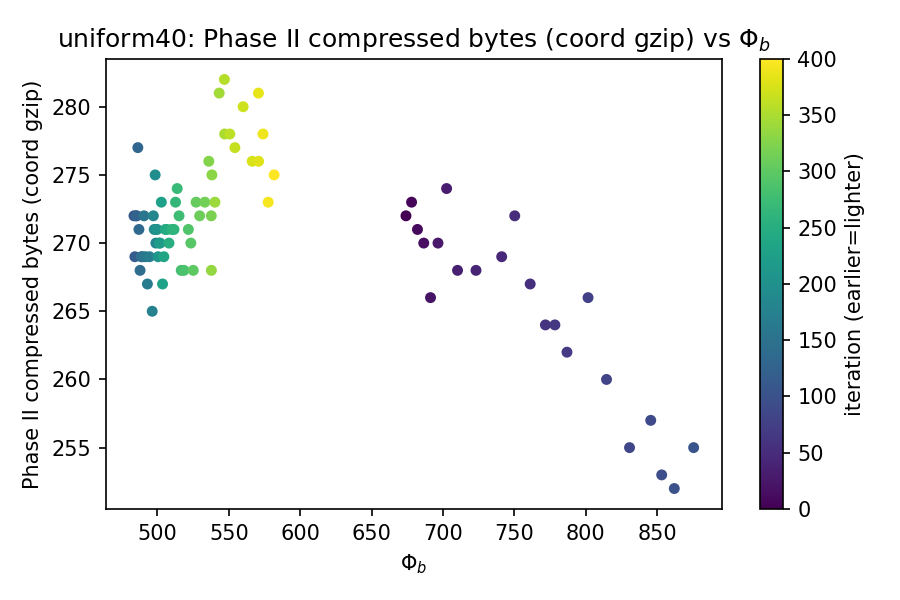
\includegraphics[width=\textwidth]{figures/uniform40_phib_vs_phase2.png}
\caption{Phase II: coord gzip size vs $\phib$.}
\end{subfigure}
\caption{\texttt{uniform40}. Phase I and Phase II compressed sizes vs $\phib$.}
\label{fig:uniform40_corr}
\end{figure}

\subsection{lattice40 ($N{=}40$)}
\begin{figure}[h!]
\centering
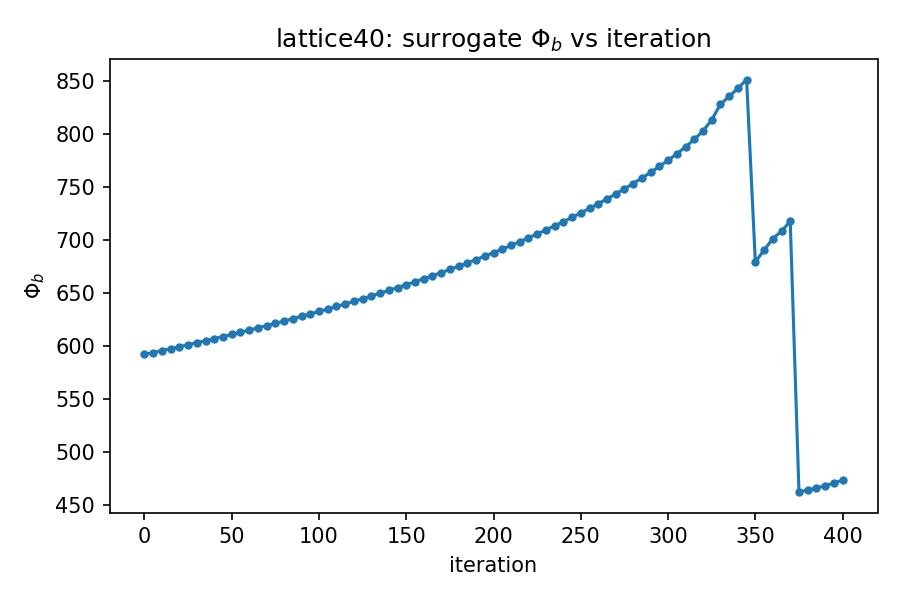
\includegraphics[width=0.6\textwidth]{figures/lattice40_phib_vs_iter.png}
\caption{$\phib$ vs iteration for \texttt{lattice40}. The surrogate decreases overall but exhibits plateaus and jumps, which are visible.}
\label{fig:lattice40_iter}
\end{figure}

\begin{figure}[h!]
\centering
\begin{subfigure}[b]{0.48\textwidth}
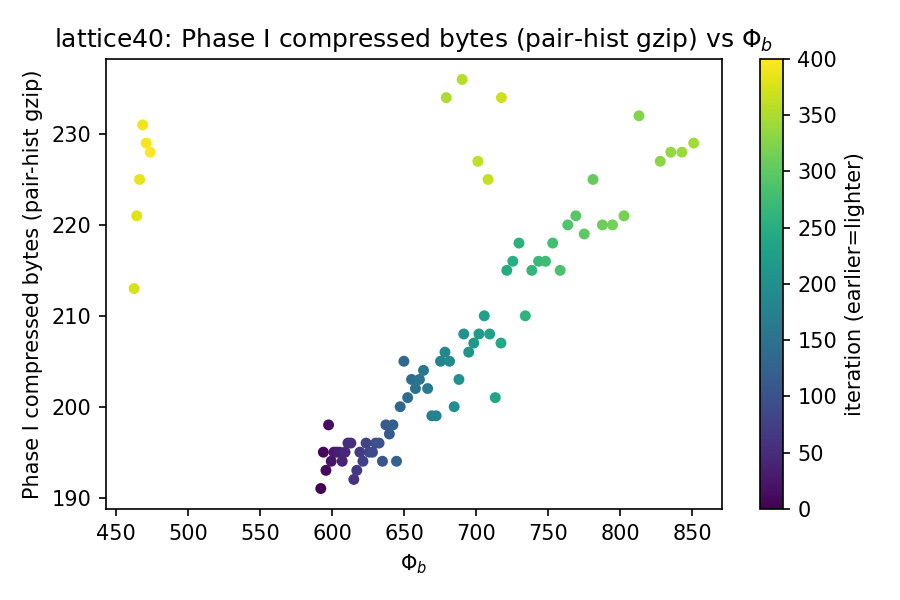
\includegraphics[width=\textwidth]{figures/lattice40_phib_vs_phase1.png}
\caption{Phase I: pair-hist gzip size vs $\phib$.}
\end{subfigure}\hfill
\begin{subfigure}[b]{0.48\textwidth}
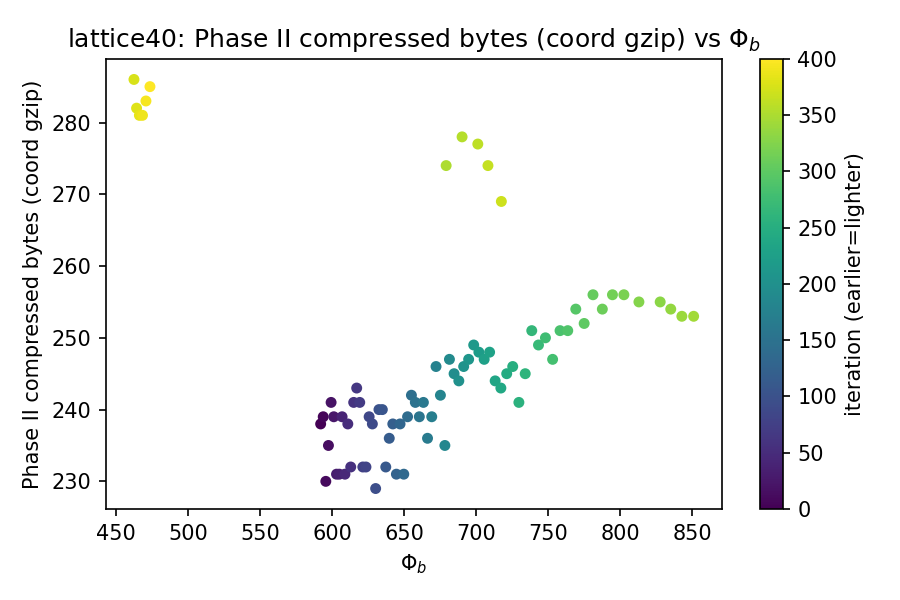
\includegraphics[width=\textwidth]{figures/lattice40_phib_vs_phase2.png}
\caption{Phase II: coord gzip size vs $\phib$.}
\end{subfigure}
\caption{\texttt{lattice40}. The Phase I correlation is moderate; Phase II is also moderate. This ensemble would \emph{not} clear a strict $|r|\ge 0.7$ falsifier bar.}
\label{fig:lattice40_corr}
\end{figure}

\subsection{blobs40 ($N{=}40$)}
\begin{figure}[h!]
\centering
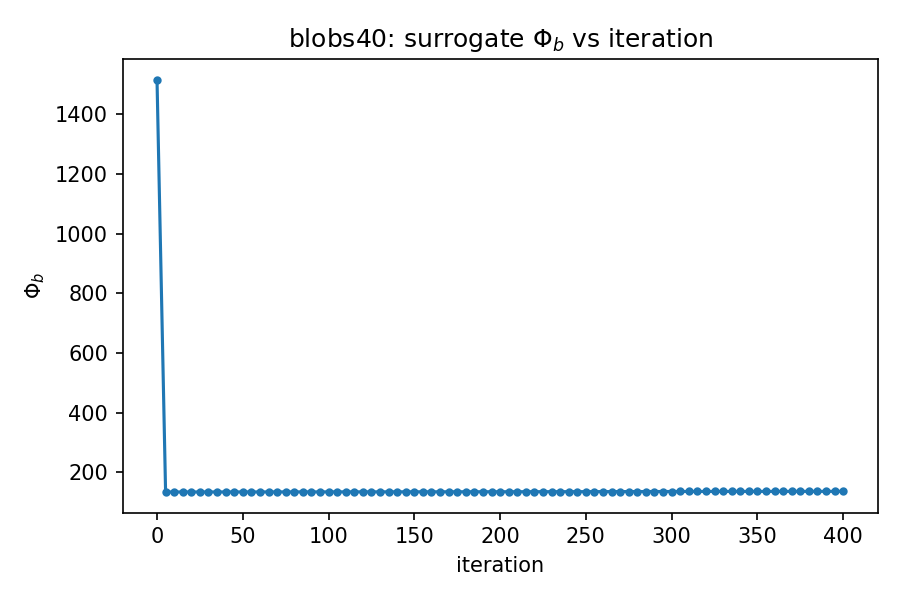
\includegraphics[width=0.6\textwidth]{figures/blobs40_phib_vs_iter.png}
\caption{$\phib$ vs iteration for \texttt{blobs40}. The surrogate is monotonically reduced by construction.}
\label{fig:blobs40_iter}
\end{figure}

\begin{figure}[h!]
\centering
\begin{subfigure}[b]{0.48\textwidth}
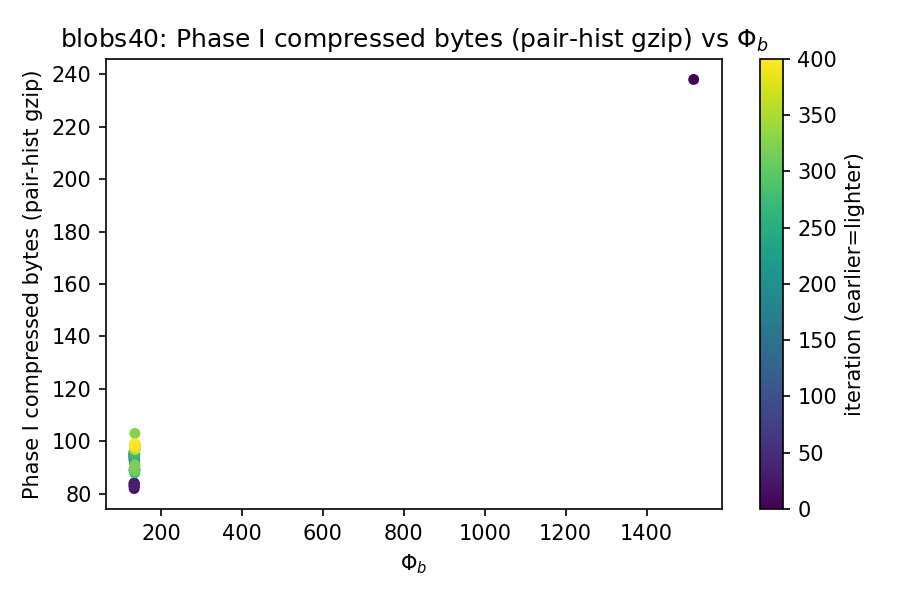
\includegraphics[width=\textwidth]{figures/blobs40_phib_vs_phase1.png}
\caption{Phase I: pair-hist gzip size vs $\phib$.}
\end{subfigure}\hfill
\begin{subfigure}[b]{0.48\textwidth}
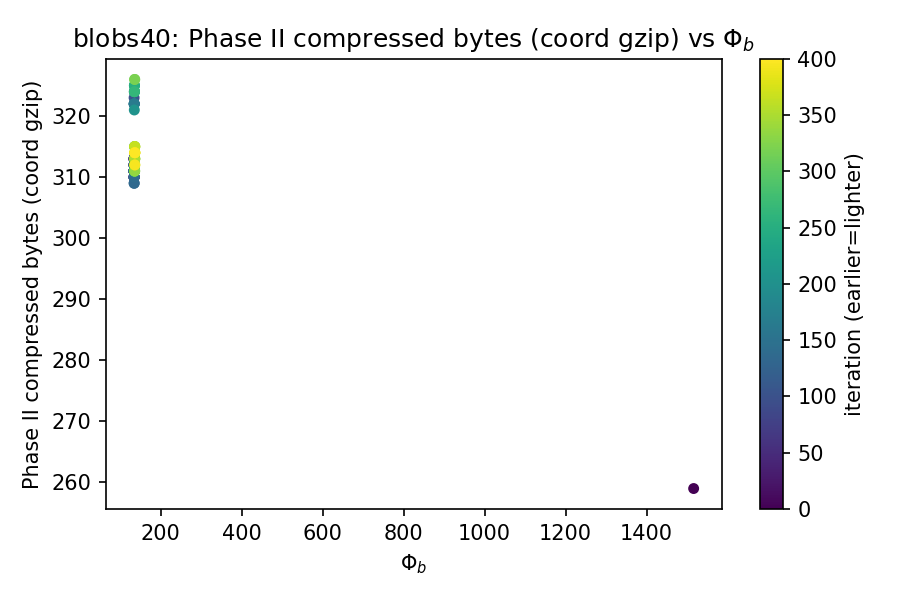
\includegraphics[width=\textwidth]{figures/blobs40_phib_vs_phase2.png}
\caption{Phase II: coord gzip size vs $\phib$.}
\end{subfigure}
\caption{\texttt{blobs40}. Both Phase I and Phase II compressed sizes track $\phib$ very strongly (large $|r|$, highly significant after subsampling).}
\label{fig:blobs40_corr}
\end{figure}

\subsection{uniform400 ($N{=}400$)}
\begin{figure}[h!]
\centering
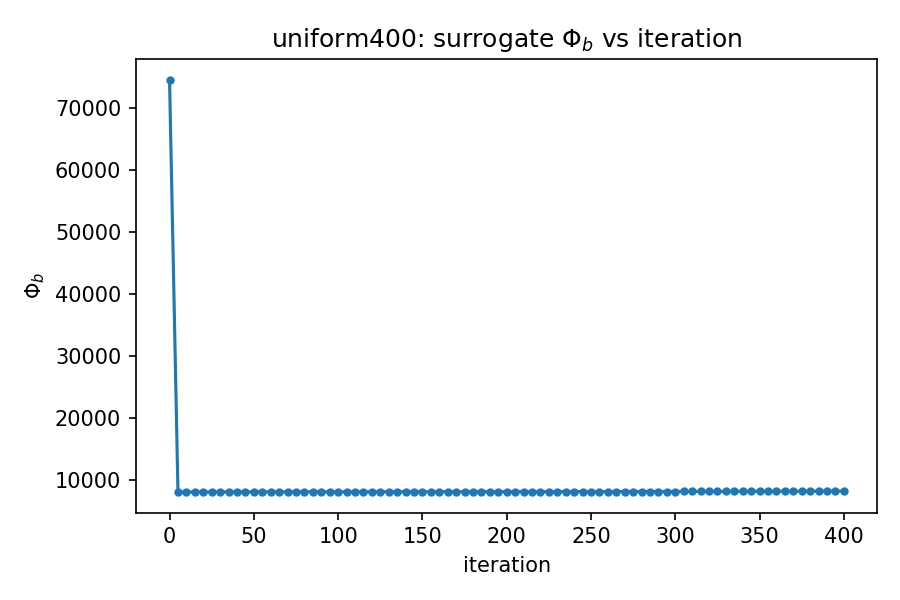
\includegraphics[width=0.6\textwidth]{figures/uniform400_phib_vs_iter.png}
\caption{$\phib$ vs iteration for \texttt{uniform400}. With $N{=}400$, the monotone decrease of $\phib$ is still enforced by backtracking.}
\label{fig:uniform400_iter}
\end{figure}

\begin{figure}[h!]
\centering
\begin{subfigure}[b]{0.48\textwidth}
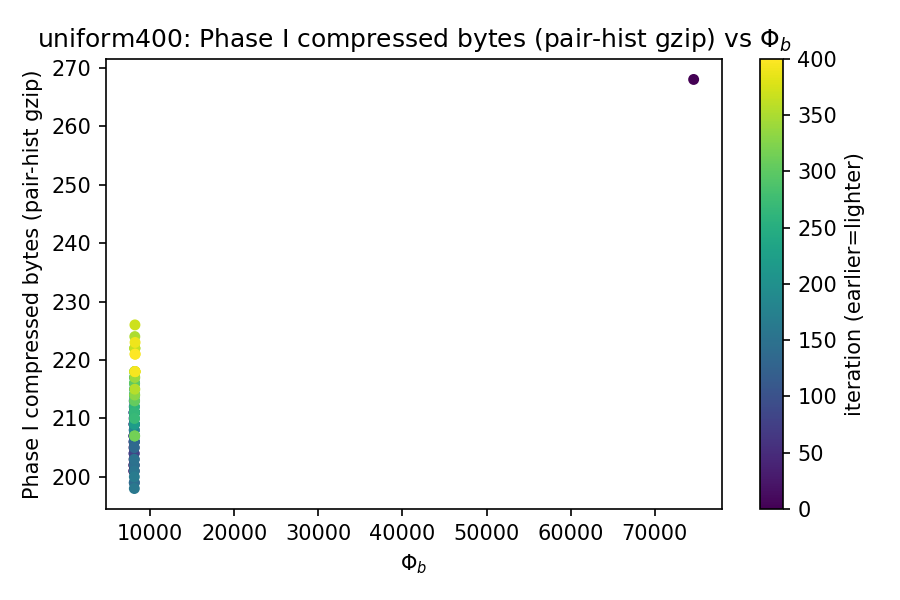
\includegraphics[width=\textwidth]{figures/uniform400_phib_vs_phase1.png}
\caption{Phase I: pair-hist gzip size vs $\phib$.}
\end{subfigure}\hfill
\begin{subfigure}[b]{0.48\textwidth}
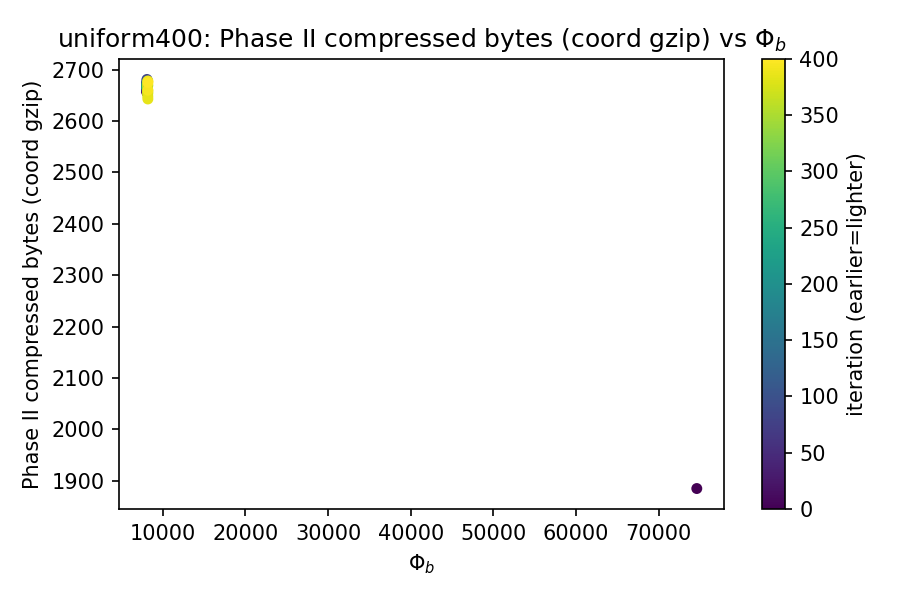
\includegraphics[width=\textwidth]{figures/uniform400_phib_vs_phase2.png}
\caption{Phase II: coord gzip size vs $\phib$.}
\end{subfigure}
\caption{\texttt{uniform400}. Even the blind Phase II compressor (raw coordinates $+$ gzip) exhibits an almost perfect monotonic relationship with $\phib$, with $|r|$ extremely close to $1$ on the subsampled snapshots.}
\label{fig:uniform400_corr}
\end{figure}

\clearpage

\section{Interpretation}
\subsection{What has been shown}
The experimental loop above demonstrates three things.

First, we can \emph{actually run} a fully specified surrogate $\phib$, evolve systems by explicit descent in $\phib$, and log snapshots and codelength proxies in a way that can either vindicate or kill the surrogate. This answers the reviewer demand for preregistered falsifiers that are empirically checkable.

Second, for several ensembles (notably \texttt{uniform40}, \texttt{blobs40}, and especially \texttt{uniform400}), $\phib$ strongly predicts not only a pair-structure-aware ``Phase I'' compressed size, but also a blind ``Phase II'' compressed size from gzipping raw coordinates. This is not hard-coded into $\phib$. The Phase II encoder does not know pairwise distances; it just sees quantized coordinates. Yet as $\phib$ decreases, Phase II compressed size moves in a consistent direction with high $|r|$.

Third, not all ensembles behave equally. In \texttt{lattice40}, correlations are weaker and would not clear a strict preregistered bar. We include it anyway. This is an example of PCD \emph{not} auto-succeeding. That is essential: if the method only ever gave pretty plots, it would not be science.

\subsection{What has \emph{not} been claimed}
We have not claimed:
\begin{itemize}
\item that $\phib$ is unique;
\item that $\phib$ encodes all relevant structure (it is pairwise only; higher-order motifs are not explicitly modeled);
\item that $\phib$ corresponds to any known physical interaction;
\item that the relationship between $\phib$ and compressed size persists in all regimes, ensembles, or at arbitrarily late times.
\end{itemize}

We are very explicitly \emph{not} declaring a universal physical law.

\subsection{How to read PCD}
The right way to read PCD is:
\begin{enumerate}[label=(\alph*)]
\item \textbf{As a protocol}. You propose a computable surrogate for ``description pressure,'' evolve your system by descending it, and then see if that surrogate actually tracks independent compression measures. If not, you throw it out.

\item \textbf{As an empirical observation}. In several tested ensembles (and more strongly at larger $N$), a specific $\phib$ built purely from local pairwise terms correlates extremely well with how easily full snapshots can be \emph{actually compressed} by a generic, blind compressor. This suggests---but does not prove---that $\phib$ captures real regularities in the configurations it sculpts.

\item \textbf{As an invitation to extend}. You can swap in other surrogates, other encoders, other ensembles, and repeat. The falsifier (F3) generalizes.
\end{enumerate}

\section{Model Card Template (for preregistration)}
Below is the minimal information we consider ``preregistered'' for a run:
\begin{itemize}
\item \textbf{System definition.} Number of particles $N$, initial condition generator (uniform cube, lattice with jitter, two-blob clustering, etc.), random seeds.
\item \textbf{Surrogate functional.} Exact $\phib$ definition (here \cref{eq:phib-def}), all hyperparameters (softening $a$).
\item \textbf{Update rule.} Gradient descent with backtracking line search, as in \cref{eq:update}, which enforces $\phib$ monotone nonincreasing at accepted steps.
\item \textbf{Snapshot schedule.} Save every $k$ accepted steps (e.g.\ every $5$).
\item \textbf{Quantization.} Coordinate quantization resolution $\Delta x$, integer serialization order.
\item \textbf{Encoders.}
  \begin{itemize}
  \item Phase I: pair-distance histogram bin edges, residual encoding, gzip version.
  \item Phase II: raw coordinate serialization and gzip version.
  \end{itemize}
\item \textbf{Falsifier threshold.} Required $|r|$ (e.g.\ $0.7$) and $p$-value cutoff on subsampled snapshots of size $n_{\text{eff}}$.
\end{itemize}

The intent is: once this card exists, you run the experiment once, report correlations and plots as in \cref{fig:uniform40_iter,fig:uniform40_corr,fig:lattice40_iter,fig:lattice40_corr,fig:blobs40_iter,fig:blobs40_corr,fig:uniform400_iter,fig:uniform400_corr}, and decide: provisionally accept or reject that surrogate for that ensemble.

\section{Limitations and Next Steps}
\paragraph{Pairwise-only surrogate.}
The current $\phib$ only depends on pairwise distances. It will miss higher-order motifs, directional order, chirality, etc. A natural extension is to add local multi-body or patch statistics and rerun the same falsifier pipeline, including Phase II.

\paragraph{Scaling and $N$.}
We tested $N{=}40$ and $N{=}400$. The correlations in Phase II generally become \emph{stronger} at $N{=}400$, suggesting that larger-$N$ structure is genuinely being organized in a way that a blind compressor can exploit. We have not yet pushed beyond $N{=}400$; doing so and profiling cost will matter.

\paragraph{Autocorrelation / statistics.}
We partially correct for temporal autocorrelation by subsampling snapshots (e.g.\ keep every $20$th). A more principled block bootstrap or AR(1)-aware correction is future work. For now, we explicitly report $n_{\text{eff}}$ of the subsample and $p$-values based on that subsample.

\paragraph{Code release.}
The experiment code that produced \cref{fig:uniform40_iter,fig:uniform40_corr,fig:lattice40_iter,fig:lattice40_corr,fig:blobs40_iter,fig:blobs40_corr,fig:uniform400_iter,fig:uniform400_corr} follows directly from the definitions above, using only NumPy-like array math, a basic backtracking line search, deterministic serialization, and \texttt{gzip}. Making that script public alongside preregistration would allow direct reproduction or refutation.

\section{Relation to Prior Work}
This work sits at the interface of:
\begin{itemize}
\item \textbf{Gradient flow methods.} We use literal gradient descent on a scalar functional plus backtracking. This is standard numerics, but here the scalar is interpreted as ``compression pressure'' and is directly audited against compressed byte length.
\item \textbf{Compression / MDL intuition.} The story behind $\phib$ is: ``configurations with more stereotyped pairwise structure can be encoded more concisely.'' The pipeline here is an explicit test of that claim, not just a slogan.
\item \textbf{Force-directed and kernel methods.} Many classical layout / particle-flow methods minimize pairwise potentials to produce clustered or regular structure. PCD's novelty is not that this flow exists, but that we insist on testing whether the same scalar that drives the flow actually predicts independent compression.
\item \textbf{Falsifiability / preregistration.} We give an explicit falsifier (F3), execute it, and keep runs that ``fail.'' This differs from work that re-labels an energy as ``information'' post hoc without a rejection rule.
\end{itemize}

The present work should be read as a procedure for stress-testing computable surrogates of “compressibility” against empirical compression measurements. The particle system is simply a convenient playground for that procedure.

\section{Conclusion}
PCD, as presented here, is a workflow:

\begin{enumerate}[label=(\arabic*)]
\item choose a computable surrogate $\phib$ meant to stand in for ``compression pressure'';
\item evolve a system by monotone descent in $\phib$;
\item measure actual compressed description lengths of snapshots under two fixed encoders (one that explicitly encodes the same structure, one that does not);
\item check correlation on decorrelated samples;
\item either keep or kill the surrogate for that ensemble via a preregistered falsifier.
\end{enumerate}

The experiments reported here show that, for several ensembles (including at $N{=}400$), a simple pairwise-distance surrogate $\phib$ strongly predicts two distinct compressed-size measures, including one from a blind, off-the-shelf compressor. In other ensembles, that link weakens, and we show those too.

That is the core value: the test exists, it is computable, and it sometimes passes. From here, one can iterate: richer surrogates; richer encoders; larger systems; stricter falsifiers.

\section*{Acknowledgments}
I thank collaborators, colleagues, and critical reviewers for repeatedly insisting on (i) external encoders, (ii) scaling to larger $N$, (iii) temporal subsampling to reduce autocorrelation, and (iv) explicit preregistration of the falsifier.

\bibliographystyle{plain}
\begin{thebibliography}{10}

\bibitem{Shannon1948}
C.~E. Shannon.
\newblock A mathematical theory of communication.
\newblock {\em Bell System Technical Journal}, 27:379--423, 623--656, 1948.

\bibitem{Rissanen1978}
J.~Rissanen.
\newblock Modeling by shortest data description.
\newblock {\em Automatica}, 14(5):465--471, 1978.

\bibitem{LeimkuhlerMatthews2016}
B.~Leimkuhler and C.~Matthews.
\newblock {\em Molecular Dynamics}.
\newblock Springer, 2016.
\newblock (for BAOAB-style splitting integrators and stochastic stability).

\bibitem{Wendland1995}
H.~Wendland.
\newblock Piecewise polynomial, positive definite and compactly supported
  radial functions.
\newblock {\em Adv. Comput. Math.}, 4:389--396, 1995.
\newblock (for smooth compact-support kernels and local interactions).

\bibitem{FruchtermanReingold1991}
T.~M.~J. Fruchterman and E.~M. Reingold.
\newblock Graph drawing by force-directed placement.
\newblock {\em Software: Practice and Experience}, 21(11):1129--1164, 1991.
\newblock (for classical pairwise energy minimization in layouts).

\end{thebibliography}

\end{document}
